

This chapter reviews some of the theoretical concepts relevant to the subsequent physics analysis. The the importance of the top quark within the Standard Model is first discussed. The modeling of physics at hadron colliders is also reviewed.

\section{Top quark physics}
The top quark was first discovered at Fermilab in 1995~\cite{Abe:1995hr}\cite{Abachi:1995iq}. As the heaviest known fundamental particle, the top quark is an important probe of the Standard Model (SM) and extensions of the SM. Before the Large Hadron Collider (LHC), the Tevatron provided the only experimental observation of the top. The LHC produces a top quark every few seconds, about a hundred times more frequently than the Tevatron. This signifigant increase in statistics allows precision measurements of the top at the LHC, which is sometimes called a ``Top Factory.'' 

\subsection{The SM}

The SM of particle physics is one of the most precisely tested and successful theories in the history of physics~\cite{peskin}. Using the mathematical framework of Quantum Field Theory (QFT), the SM relies upon the conservation of a symmetry called gauge invariance and describes interactions between particles via the strong, weak and electromagnetic forces.  

Tables~\ref{t:pspincharge}-\ref{t:pmass} summarize the properties of the fundamental particles of the SM: three generations of quarks, three generations of leptons, gauge bosons, and the recently discovered Higgs boson. With the discovery of the Higgs boson in 2012, all predictions of the SM have been verified and found to be self-consistent up to the Planck scale ($10^{15-19}$ \gev). 

Because of its large mass, the top quark plays a special role in the SM. The top mass is about the same as a gold atom nucleus, 40 times larger than the next heaviest quark and $10^5$ times heavier than the lightest quark. The mass of the top quark has been precisely measured in different decay channels at both the LHC and the Tevatron. Figure~\ref{fig:topmass} shows a recent summary of these measurements, which can be combined to give a world average of $173.34 \pm 0.76$ for the top quark mass.

 The top has a very short lifetime ($\sim 5 \e{-25}$ s), so it is the only quark that decays before it can form a hadron with other quarks. This unique property means that the top is the only ``bare'' quark that can be accessed at the LHC. The top is also the only quark with Yukawa coupling to the Higgs boson of order unity. Thus, accurately measuring its properties (mass, coupling, cross section, branching ratios) provides an important information about Quantum Chromodynamics (QCD), the SM description of interactions between quarks via the strong force. 

\subsection{Beyond the SM}
In addition to providing a test of the SM, the top quark may also provide a window to physics at higher energy scales beyond the SM.

The top quark is important in aesthetic problem with the Higgs mass known as the hierarchy problem or fine tuning. The Higgs mechanism provides an explanation for electroweak symmetry breaking and acquisition of mass by other SM particles. As a scalar particle, the Higgs receives higher-order corrections to its physical (measured) mass from interactions with fermions, gauge bosons and itself. These corrections are on the order of the Planck scale, $\mathcal{O}(\Lambda^2 \approx 10^{30-38} \gev)$, while the observed mass is class to the electroweak scale, $\mathcal{O}(100 \mev)$. Thus, in order to obtain the observed mass without introducing new physics, there must be an unnatural canceling. Since the dominant higher-order correction to the Higgs mass comes from the top, precisely measuring the top's mass and other properties may provide insight to this problem. 

In addition to the hierarchy problem, there are several other open questions which cannot be explained by the SM. The SM does not account for the 85\% of our universe made up of \textit{dark matter} particles, or provide an explanation for the observed asymmetry between matter and anti-matter. The SM also does not account for the observed non-zero mass of neutrinos or have a way to incorporate gravitational interactions.

Theorists have formulated many extensions to the SM that address these puzzles. Perhaps the most widespread, Supersymmetry (SUSY)~\cite{susy} proposes an additional superpartner for every particle in the SM. SUSY is especially popular because it naturally contains a light, stable, neutral dark matter candidate and solves the hierarchy problem. Diagrams from superpartners remove the need to fine tune the Higgs mass. Since SUSY has not been observed, the superpartners of SM particles must have different masses, and SUSY has to be a broken symmetry. However, in order to satisfactorily solve the hierarchy problem, the superpartners with the largest contributions to the Higgs mass must be $\mathcal{O}(\tev)$. This means that they should be discoverable at the LHC.

Another popular SM extension, called the Randall-Sundrum model~\cite{Lillie:2007yh}, posits an extra dimension in which gravity would propagate. This model includes a new particle, a Kaluza-Klein gluon, that propagates into the extra dimension and decays into a top quark pair.
%COULD ADD MORE ABOUT WHY SIGNALS IMPOR. See a thesis

Many of the signals for new physics are dominated by the top quark since heavier particles are more sensitive to higher energy scales.  The top pair production analyzed in this thesis is important as a background for \ttbar resonances~\cite{ATLAS-CONF-2015-009} and other searches~\cite{Aad:2014kra}.



\section{Top quark production at the LHC}

In $pp$ collision at the LHC, top quarks are mostly produced in pairs through the leading order QCD processes  $gg \rightarrow \ttbar$ and $q\bar{q} \rightarrow \ttbar$. The Feynman diagrams for these processes are shown in Figure~\ref{fig:ttdiag}. At Tevatron with $p\bar{p}$ collisions, \ttbar production was dominated by quark annihilation ($\sim 85$\%). At the LHC, the higher collision energy and lack of valence anti-quarks in the proton result in gluon-fusion dominated \ttbar production ($\sim 85$\%)~\cite{PDG}. The total \ttbar cross-section has been computed at next-to-next-to leading order (NNLO) with next-to-next-to-leading-log soft gluon resummation (NNLL) in Ref.~\cite{Czakon:2013goa} with a final theoretical uncertainty of $\sim\ 3 \%$ and found to agree with experimental measurements. Figure~\ref{fig:ttxsec} compares this calculation with measurements made at both in the LHC and Tevatron in various decay channels.

Top quarks can also be produced singly via electroweak processes. Because the weak coupling is much smaller than the strong coupling, fewer quarks are produced singly than in pairs. The Feynman diagrams for single top production are shown in Figure~\ref{fig:tdiag}. Single production can mediated by virtual $s$-channel and $t$-channel $W$-bosons. These production channels provide sensitivity to physics beyond the SM. Single tops are also produced in association with a $W$-boson ($Wt$-associated production). While negligible at the Tevatron, at the LHC, $Wt$-associated production provide a sizeable contribution to single top production. The inclusive cross-section for $s$-channel, $t$-channel and $Wt$-associated single top production has been computed to NNLO. This calculation is compared with the ATLAS experimental measurements of each channel in Figure~\ref{fig:txsec}.

\section{Top quark decays}
At lowest order in the SM, the top quark can only decay to a $W$ boson and a down-type quark: $t \rightarrow qW$ where $q=b,s,d$. The rate of each of these decays is proportional to the square of the Cabibbo-Kobayashi-Masakawa (CKM) matrix, $|V_{tq}|^2$. Measured from experiment, the CKM matrix governs quark mixing in flavor-changing weak decays~\cite{PDG}.

Weak hadron decays and the unitiary of the CKM matrix constrain the value of $0.9990 < |V_{tb}| < 0.9992$ at the 95\% C.L~\cite{Chetyrkin:1999ys}. Top quarks nearly always decay with $t \rightarrow Wb$.

Experimentally, the decay modes of \ttbar are distinguished by the decay  of the two $W$-bosons:
\begin{list}
\item[All hadronic] Both $W$ boson decay to quark pairs: $\ttbar \rightarrow WbWb \rightarrow 2b4q$. Because there are 6 quarks in the final state, this channel has a large multi-jet background, which can be difficult to subtract. 

\item[Semi-leptonic] One $W$ boson decays to a quark pair and the other decays to a lepton and neutrino: $\ttbar \rightarrow WbWb \rightarrow 2b2q \ell \nu$. 


\item[All hadronic] Both $W$ boson decay to quark pairs: $\ttbar \rightarrow WbWb \rightarrow 2b4q$. Because there are 6 quarks in the final state, this channel has a large multi-jet background, which can be difficult to subtract. 


\end{list} 

\section{Monte Carlo prediction}
Since the mass of the top quark is above $\Lambda_{QCD}$, top quark production at the LHC can be predicted by perturbative QCD. The \ttbar ($\sigma_{\ttbar}$) cross section is a convolution of the partonic cross section ($\qqbar, qq \rightarrow \ttbar$)and the parton distribution functions (PDFs):

\begin{equation}
\sigma_{\ttbar}(s, m_{t}) = \sum_{i, j} \int^1_0 dx_i  \int^1_0 dx_j f_i \left(x_i, \mu_F^2 \right) f_j\left(x_j, \mu_F^2 \right) \times \hat{\sigma}_{ij} \left( \hat{s}, m_{t}, \alpha_s \left(\mu_R \right), \mu_R,  \right)
\end{equation}


\begin{table}
\begin{tabular}[b]{|l||ccc|c|c|}
\hline
           & \multicolumn{3} {c|} {particles} & spin & electric charge \\
\hline
\hline
               & $(u,d)_L$ & $(c,s)_L$ & $(t,b)_L$ & $(\frac{1}{2},\frac{1}{2})$ & $(+\frac{2}{3},-\frac{1}{3})$ \\
Quarks         & $u_R$     & $c_R$     & $t_R$     & $\frac{1}{2}$               & $+\frac{2}{3}$                \\
               & $d_R$     & $s_R$     & $b_R$     & $\frac{1}{2}$               & $-\frac{1}{3}$                \\
\hline
\multirow{2} {*} {Leptons} & $(\nu_e, e^-)_L$ & $(\nu_{\mu},\mu^-)_L$ & $(\nu_{\tau}, \tau^-)_L$ & $(\frac{1}{2},\frac{1}{2})$ & (0,-1) \\
                           & $e^-_R$          & $\mu^-_R$             & $\tau^-_R$               & $\frac{1}{2}$               & -1     \\
\hline
                           & \multicolumn{3} {c|} {$g$}               & 1 & 0 \\
Gauge bosons               & \multicolumn{3} {c|} {$W^{\pm}$ and $Z$} & 1 & $\pm$1 and 0 \\
                           & \multicolumn{3} {c|} {$\gamma$}          & 1 & 0 \\
\hline
Scalar boson               & \multicolumn{3} {c|} {$H$} & 0 & 0 \\
\hline 
% 
\end{tabular}
\label{t:pspincharge}
\caption{Spin and charge of particles in the SM.}
\end{table}
\begin{table}
\begin{tabular}[b] {|l|l|l|}
& Particle & Mass  \\
%%%%%%%%%%%%%%%%%%%%%%%%%%%%
\hline
\hline
\multirow{3} {*} {Leptons} & $e$ & 0.511 MeV  \\
& $\mu$ & 105 MeV \\
& $\tau$ & 1777 MeV \\
\hline \hline
 \multirow{3} {*} {Gauge bosons} & $W^{\pm}$ & 80.2 GeV \\
& $Z$ & 91.19 GeV  \\
\hline
& $H$ & 126 GeV \\
\hline \hline
 \multirow{3} {*} {Quarks} & up ($u$) & 1.7-3.3 \mev \\
& down ($d$) & 4.1-5.8 \mev  \\
\hline
& charm ($c$) & 1.18-1.34 \gev  \\
& strange ($s$) & 70-120 \mev \\
\hline
& top ($t$) & $173.34 \pm 0.76$  \gev  \cite{ATLAS:2014wva}\\
& bottom ($b$) & $4.18 \pm 0.03$ \gev \\
\hline \hline
\multirow{3} {*} {Hadrons} & $p$ & 938 MeV\\
& $n$ & 939 MeV  \\
& $\pi^{\pm}$ & 139.6 MeV \\
& $\pi^0$ & 135.0 MeV  \\
\hline
\end{tabular}
\label{t:pmass}
\caption{Mass of particles in the SM, taken from Ref.~\cite{PDG}.}
\end{table}

\begin{figure}
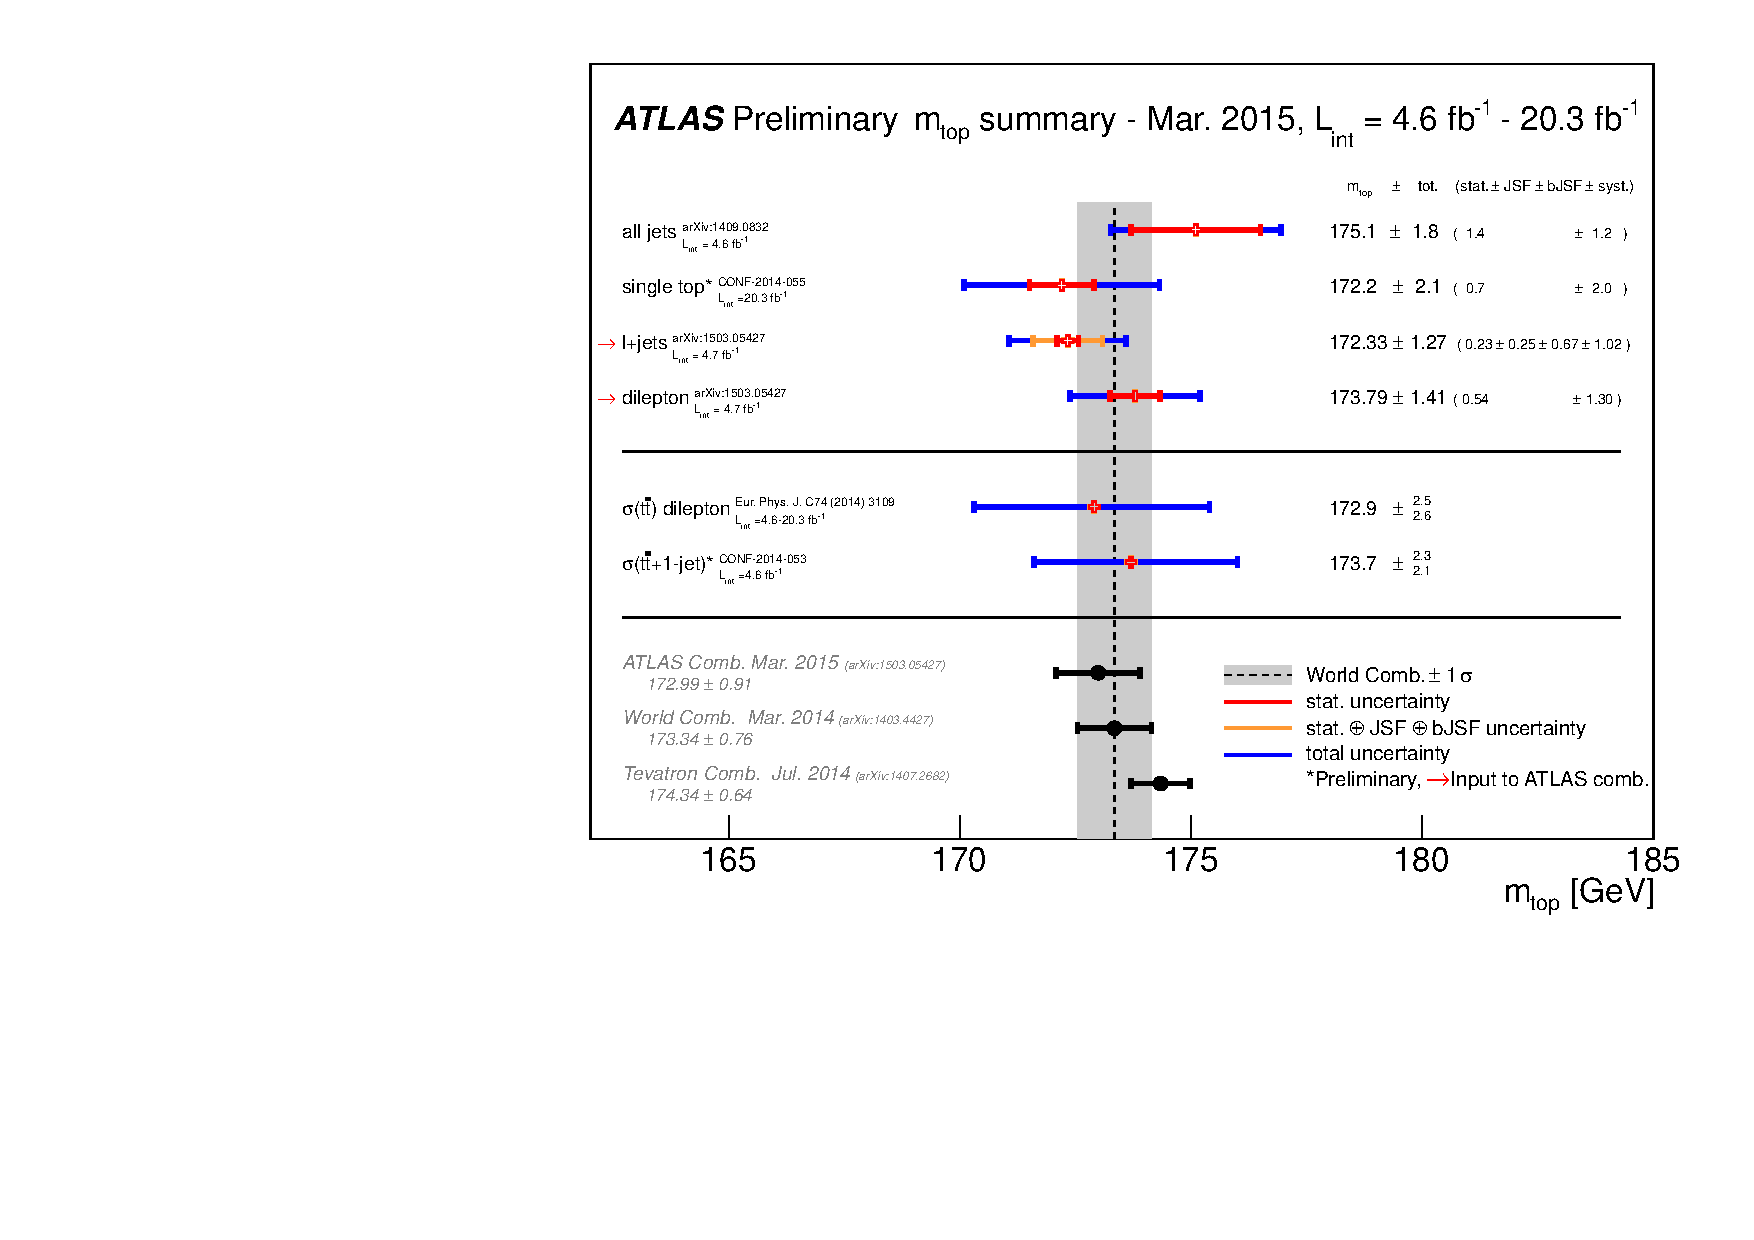
\includegraphics[width=\textwidth]{fig/mtopSummary_All.pdf}
\caption{Summary of the ATLAS direct $m_{top}$ measurements. The results are compared with the ATLAS, Tevatron and Tevatron+LHC $m_{top}$ combinations. For each measurement, the statistical uncertainty, the sum of the remaining uncertainties are reported separately. The JSF, bJSF contributions are statistical in nature and apply to analyses performing in-situ (top quark pair base) jet energy calibration procedures.}
\label{fig:topmass}
\end{figure}

\begin{figure}
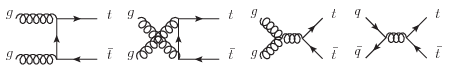
\includegraphics[width=\textwidth]{fig/fig_ttbar.png}
\caption{Feynman diagrams for \ttbar production at leading order QCD}
\label{fig:ttdiag}
\end{figure}

\begin{figure}
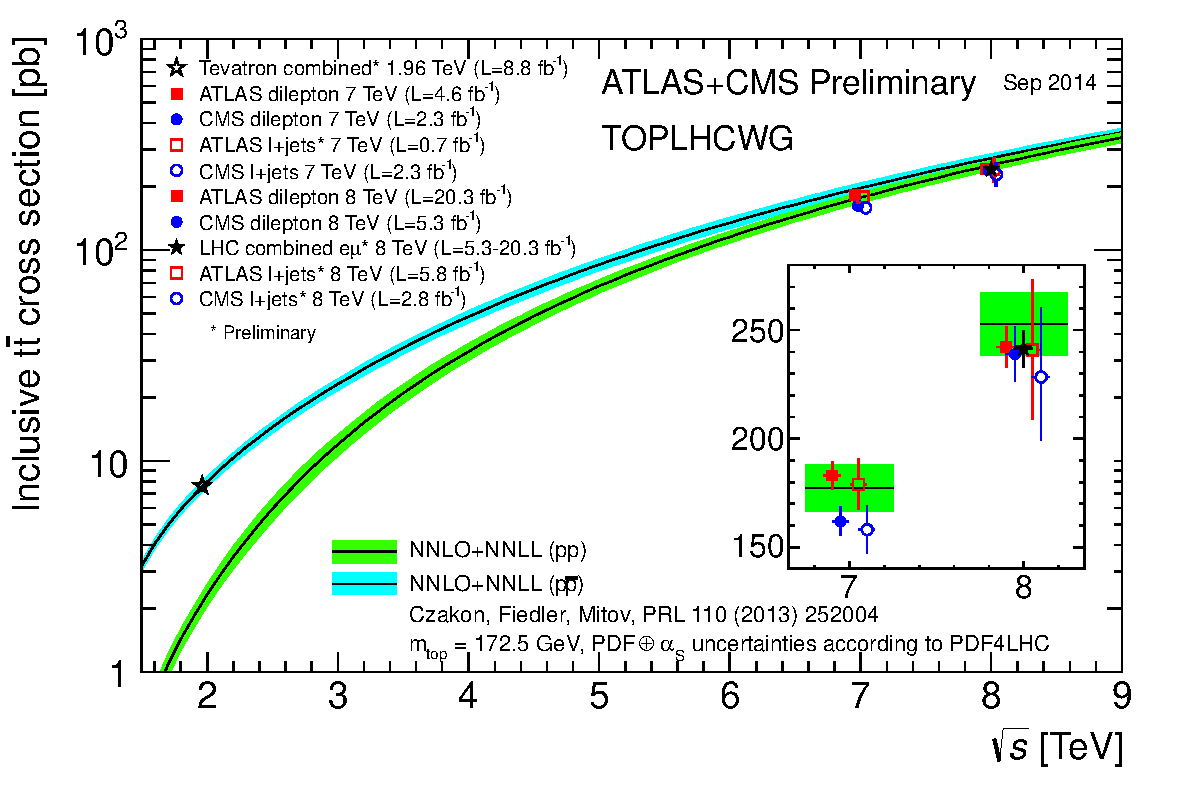
\includegraphics[width=\textwidth]{fig/tt_xsec_vsroots.pdf}
\caption{Summary of LHC and Tevatron measurements of the top-pair production cross-section as a function of the centre-of-mass energy compared to the NNLO QCD calculation complemented with NNLL resummation (top++2.0). The theory band represents uncertainties due to renormalisation and factorisation scale, parton density functions and the strong coupling. The measurements and the theory calculation is quoted at $m_{top}$=172.5 GeV. Measurements made at the same centre-of-mass energy are slightly offset for clarity.}
\label{fig:ttxsec}
\end{figure}

\begin{figure}
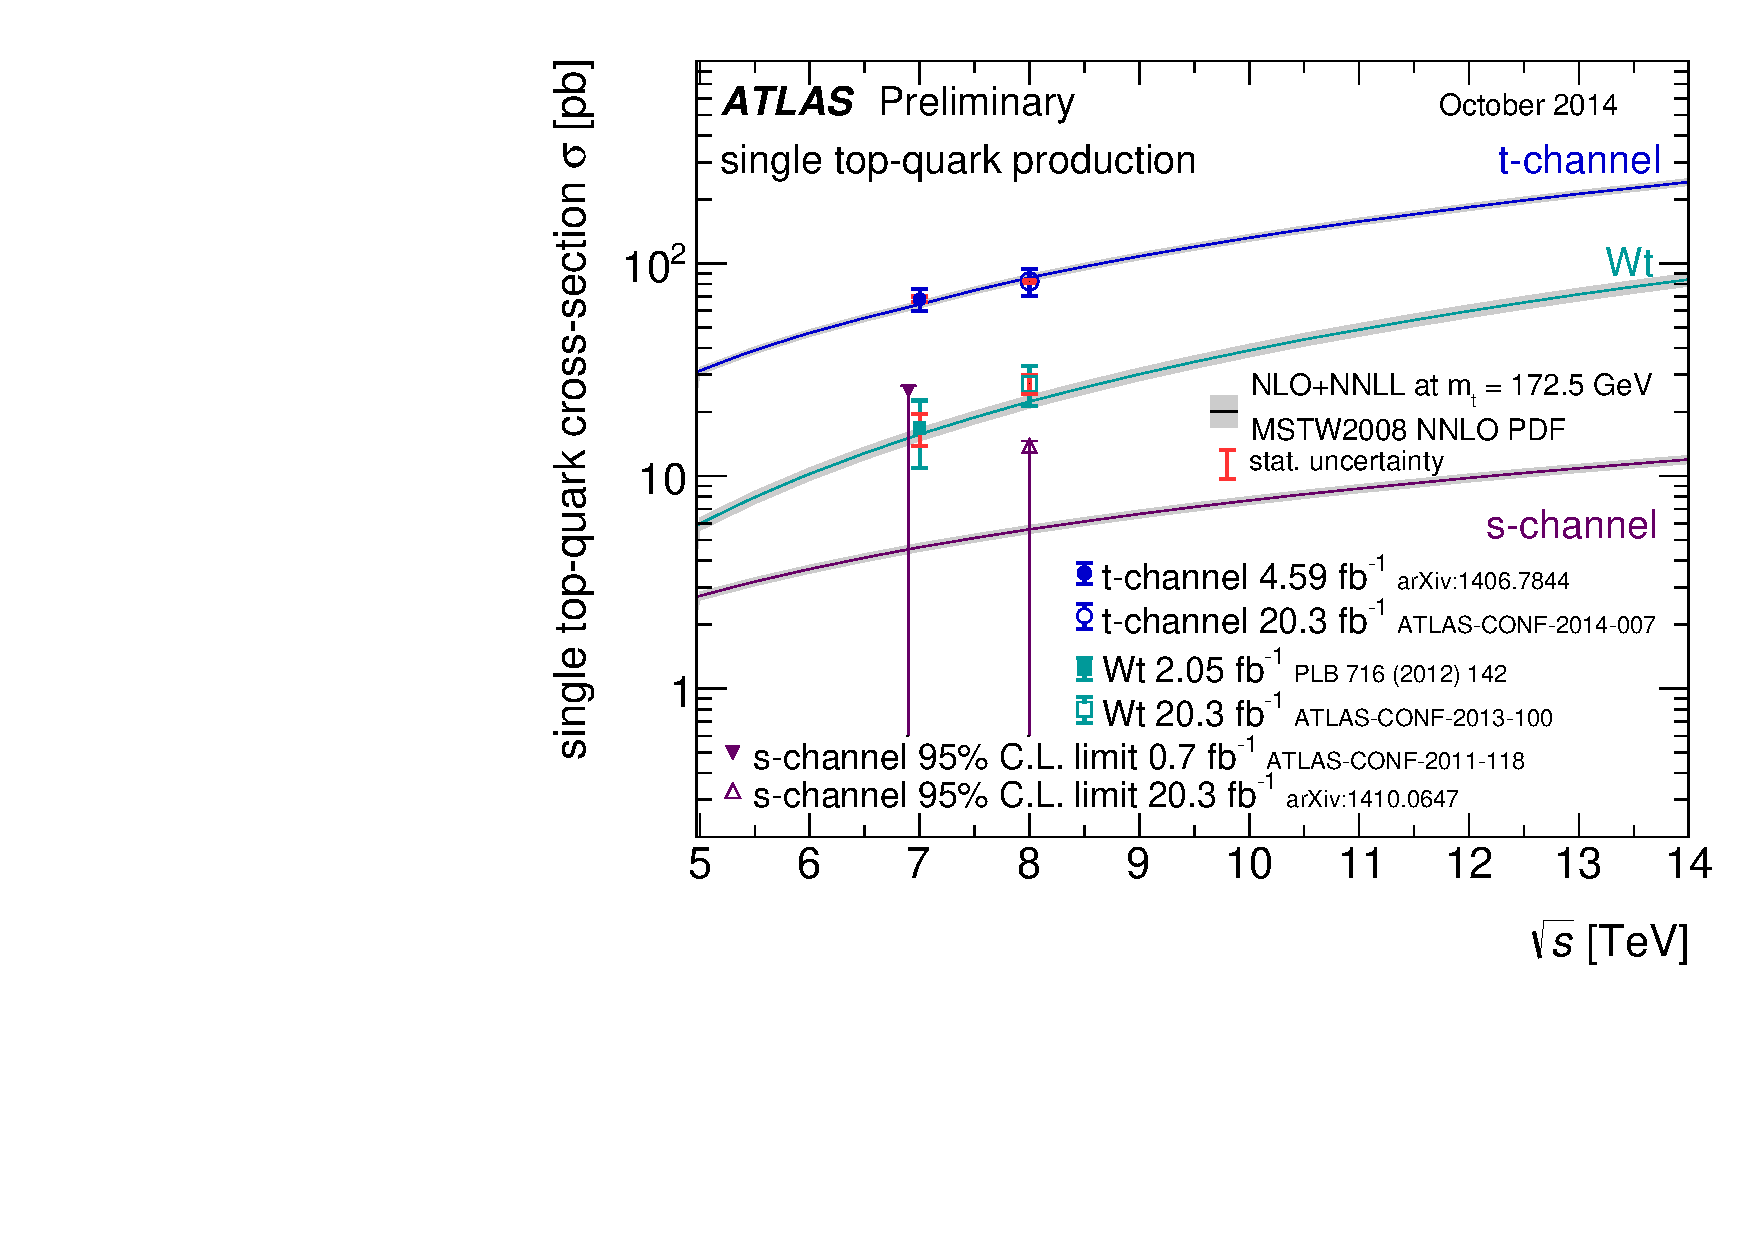
\includegraphics[width=\textwidth]{fig/singletop_allchanvsroots_ATLASonly.pdf}
\caption{Summary of ATLAS measurements of the single top production cross-sections in various channels as a function of the center of mass energy compared to a theoretical calculation based on NLO QCD complemented with NNLL resummation. For the $s$-channel only an upper limit is shown.}
\label{fig:txsec}
\end{figure}

\begin{figure}
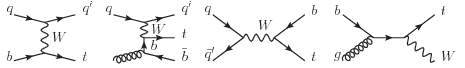
\includegraphics[width=\textwidth]{fig/fig_singletop.png}
\caption{Feynman diagrams for single top quark production at leading order QCD. From left to right: $t$-channel production as flavor excitation; $t$-channel production as $W$-gluon fusion; $s$-channel production; $Wt$-channel production.}
\label{fig:tdiag}
\end{figure}
